\documentclass[a4paper,11pt]{article}
\input{/home/tof/Documents/Cozy/latex-include/preambule_doc.tex}
\input{/home/tof/Documents/Cozy/latex-include/preambule_commun.tex}
\newcommand{\showprof}{show them}  % comment this line if you don't want to see todo environment
\setlength{\fboxrule}{0.8pt}
\fancyhead[L]{\fbox{\Large{\textbf{Loc 01}}}}
\fancyhead[C]{\textbf{Principe de la géolocalisation}}
\newdate{madate}{10}{09}{2020}
%\fancyhead[R]{\displaydate{madate}} %\today
\fancyhead[R]{Seconde - SNT}
\fancyfoot[L]{\vspace{1mm}Christophe Viroulaud}
\AtEndDocument{\label{lastpage}}
\fancyfoot[C]{\textbf{Page \thepage/\pageref{lastpage}}}
\fancyfoot[R]{\includegraphics[width=2cm,align=t]{/home/tof/Documents/Cozy/latex-include/cc.png}}

\begin{document}
\begin{center}
    \framebox{Comment repérer une position sur Terre?}
\end{center}
\section{Repérage sur Terre}
Deux cercles de référence :
\begin{itemize}
    \item l’équateur,
    \item le méridien de Greenwich.
\end{itemize}
\begin{center}
    \centering
    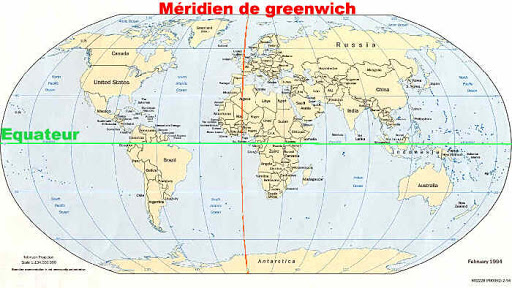
\includegraphics[width=8cm]{ressources/greenwich.jpg}
    \captionof{figure}{Cercles de référence}
    \label{greenwich}
\end{center}

Pour repérer une position M sur la Terre en trois dimensions on utilise des angles (figure \ref{geoloc}):
\begin{itemize}
    \item sa longitude, angle entre le méridien de Greenwich et le méridien passant par M,
    \item sa latitude, angle entre l’équateur et le parallèle passant par M.
\end{itemize}
\begin{center}
    \centering
    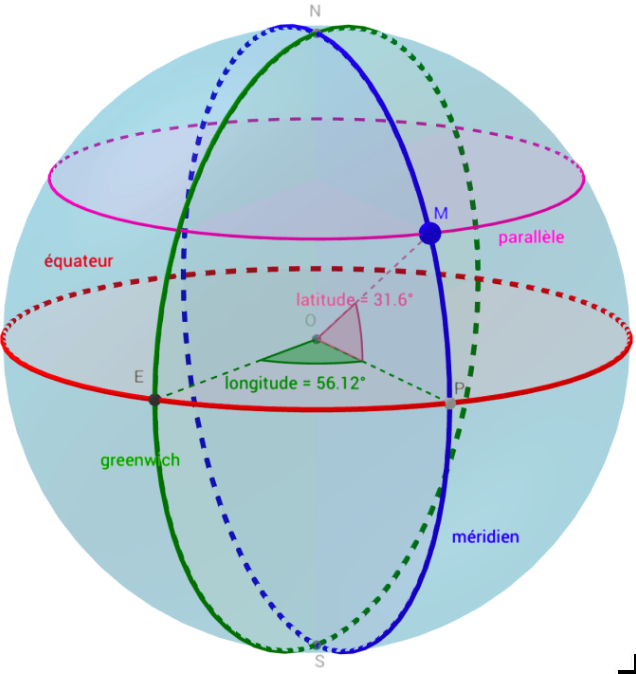
\includegraphics[width=6cm]{ressources/geoloc.png}
    \captionof{figure}{Latitude et longitude}
    \label{geoloc}
\end{center}
Dans la figure \ref{geoloc} les coordonnées du point M sont:
\begin{itemize}
    \item latitude: 31,6°N
    \item longitude: 56,12°E
\end{itemize}
\begin{center}
    \centering
    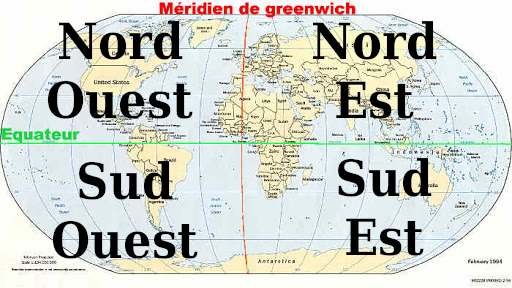
\includegraphics[width=6cm]{ressources/zone.png}
    \captionof{figure}{Zones des latitudes et longitudes}
    \label{zone}
\end{center}
\section{Se repérer grâce à des satellites}
\subsection{Principe: la trilatération}
Pour se repérer sur Terre on positionne des satellites artificiels autour du globe (figure \ref{gps0}).
\begin{center}
    \centering
    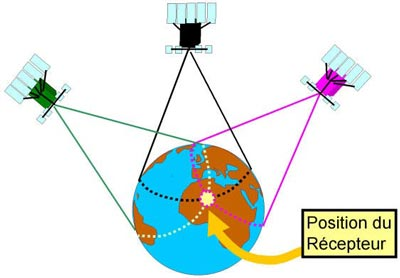
\includegraphics[width=6cm]{ressources/gps0.jpg}
    \captionof{figure}{Un système de satellites}
    \label{gps0}
\end{center}
Chaque satellite envoie sa position très précise dans toutes les directions. Le récepteur sur Terre (un smartphone, une montre connectée\dots) est positionné sur la sphère centrée sur le satellite.
\begin{center}
    \begin{tabular}{ccc}
        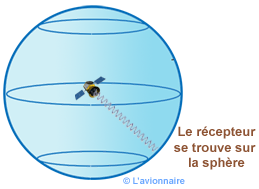
\includegraphics[width=5cm]{ressources/gps1.png}
        &
        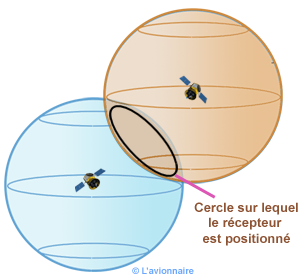
\includegraphics[width=5cm]{ressources/gps2.png}
        &
        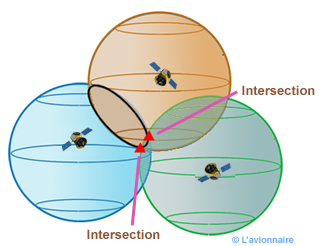
\includegraphics[width=5cm]{ressources/gps3.png}
        \\
    \end{tabular}
\end{center}
\begin{aretenir}[Remarque]
En réalité, on utilise un quatrième satellite pour gagner en précision, avoirs des informations sur l'altitude\dots
\end{aretenir}
\subsection{Différents systèmes}
On parle communément de GPS (\emph{Global Positioning System}) car c'est le premier système mis en place par la Défense américaine en 1973. Il utilise 31 satellites. Les informations fournies sont précises à l'ordre du mètre mais cette précision était d'abord réservée à un usage militaire. La population civile ne pouvait obtenir une précision qu'à plusieurs centaines de mètres. Cette limitation a été levée au début des années 2000.

\end{document}